\chapter{Experiments}\label{chapter:experiments}




\section{Experimental Setup: Ball Screw Drive}
In order to evaluate different predictive maintenance approaches, data from a DMG DMC 55H duoblock milling machine of the manufacturer DMG Mori were collected. The machine tool’s spindle and housing, as well as the machine tool table, rotatory axes, peripherals, the cladding and the machine tools housing were removed. The TNC control iTNC530 HSCI from Heidenhain GmbH was used.

The focus of the experiments is to investigate different levels of abrasion in the linear guiding shoes (LGSs)and ball screw drives (BSDs) of the machine. The machine component damages are separated in different types, pitting (P) and no pitting (C). Generally, no pitting was detected for the LSGs. The health condition state of each component is specified by one letter and two digits. The letter indicates the damage type, the first digit the component’s preload class and the second digit the number of the observation. Fig. \ref{fig:experimental_setup} shows the experimental setup. The investigation focuses on the moving hanger assembly of the machine tool. The machine tool can be moved in the three spatial directions. The experiments are restricted to the movement of the machine tool along the x-Axis. For this reason just the single threaded shaft of the BSD and the two counterparts each belonging to one of the two LGSs are supervised.

\begin{figure}[htpb]
  \centering
  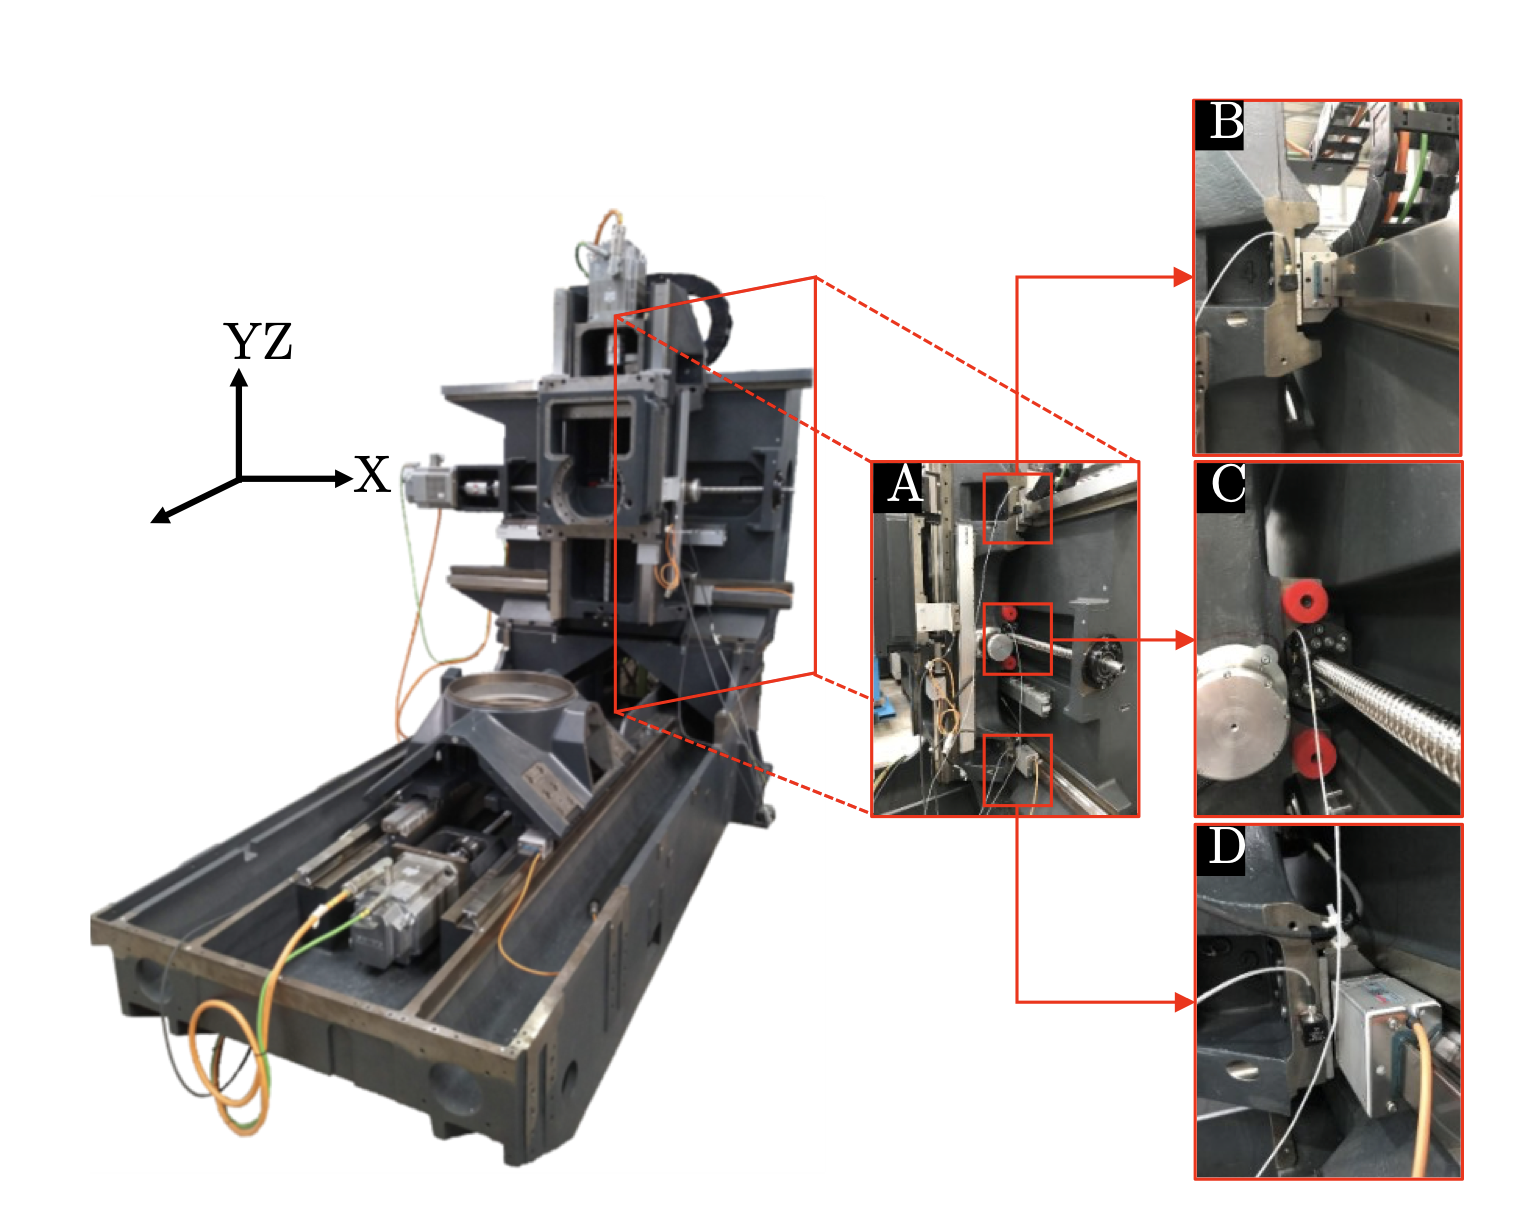
\includegraphics[width=0.9\textwidth]{experimental_setup}
  \caption {Experimental Setup: A: side-view of the machine, B: Upper LGS, C: BSD, C: Lower LGS}
  \label{fig:experimental_setup}
\end{figure}
\FloatBarrier 


An overview over the the tracked health condition states of the LGSs and BSDs is visualized in table \ref {tab:BSDs_states} and table \ref {tab:LGSs_states}. The ID specifies the damage class, the component the affected parts of the industrial machine and the preload in N the force measured in the LGSs and BSDs. Since just two LGSs consisting of two parts and the threaded shaft of the BSD are supervised each BSD damage ID maps to one component and each LGS damage ID maps to four components. 


\begin{center}
\begin{longtable}{||c c c||} 
 \hline
 ID & component name & preload in N \\ [0.5ex] 
 \hline
 P1 & 721-14448-6-G6 & 2 070 \\ 
 P2 & 721-14448-4-G4 & 2 160 \\ 
 C11 & 721-14448-3-G3 & 2 950 \\ 
 C12 & 721-95859-4 & 845 \\ 
 C21  & 721-14448-1-G1 & 1 450 \\ [1ex] 
 C22  & 721-95859-2 & 1 293 \\ [1ex] 
 C31  & 721-14448-2-G2 & 2 390 \\ [1ex] 
 C32  & 721-95859-3 & 2 328 \\ [1ex] 
 C33 & 721-95859-1 & 2 031 \\ [1ex]
   \hline
\caption {BSDs states}
\label {tab:BSDs_states}
\end{longtable}
\end{center}


\begin{center}
\begin{longtable}{||c c c||} 
 \hline
 ID & component name & preload in  \\ [0.5ex] 
 \hline\hline
 C1 & C1 & 4 060 \\ 
    & C2 & 4 430 \\ 
    & C3 & 4 430 \\
    & F1 & 3 880 \\ 
 \hline
 C2 & B1 & 8 860 \\ 
    & B2 & 9 700 \\ [1ex] 
    & B3 & 9 070 \\ [1ex]
    & E1 & 8 230 \\ [1ex]
 \hline
 C3 & A9 & 13 470 \\ 
    & A10 & 14 530 \\ [1ex] 
    & A11 & 12 840 \\ [1ex]
    & D3 & 12 840 \\ [1ex]
 \hline
\caption {LGSs states}
\label {tab:LGSs_states}
\end{longtable}
\end{center}

 Via TNC Scope internal control data and via TNC Opt internal control data is accessed. Three triaxial Kistler 8762A10 piezo-eletric accelerometers were used to track accelerations in the spatial directions X.

\section{Dataset: Ball Screw Drive}
In order to keep the reproducibility of this experiment a defined test cycle, which is defined in fig. \ref{fig:test_cycle}, was used to record the data. Machine data is collected during constant speed, direction change and sweep excitement along the machine tools X-axis. During the constant speed excitement the machine tools are moved along the whole axis  ($\Delta x$ = 600mm) back and forth. In the direction change excitation the movement of the machine tools is restricted to a small part of the axis ($\Delta x$ = 1mm) and the directions are changed with a high frequency. In the sweep excitement the motor, moving the machine tools along the different axis, receives a target speed in form of a sine sweep. Before recording data, the machine is warmed up in order to create equivalent circumstances for each run. For this reason constant speed excitement is applied for 60 min. 


\begin{figure}[htpb]
  \centering
  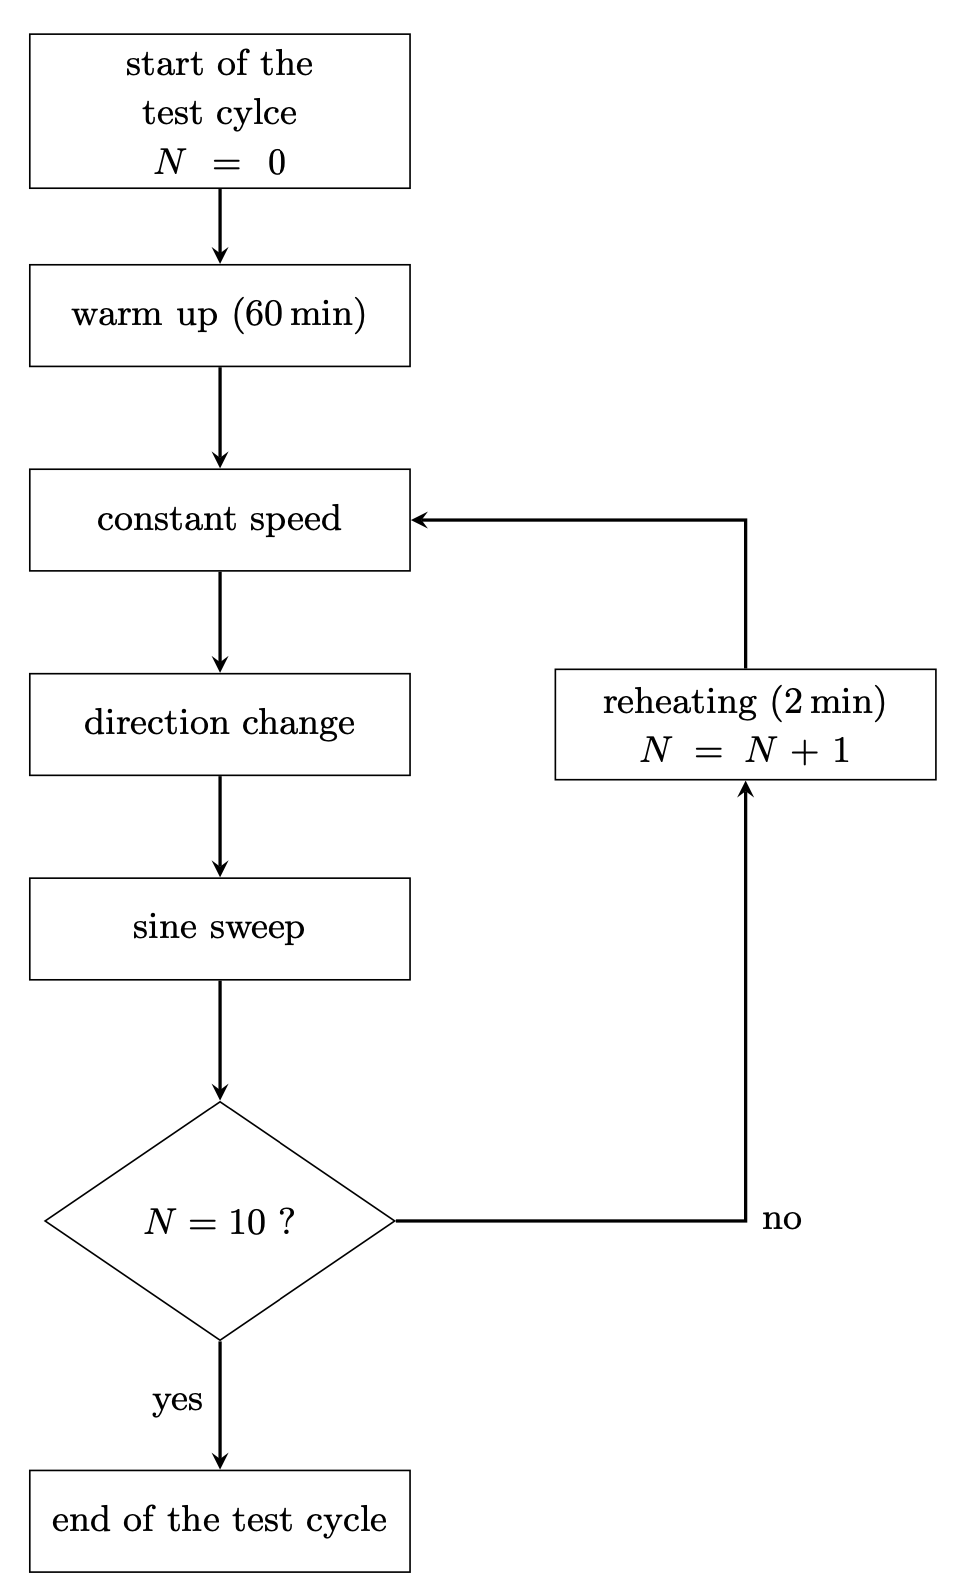
\includegraphics[width=0.7\textwidth]{test_cycle}
  \caption {Flow chart explaining the test cycle used in the presented dataset}
  \label{fig:test_cycle}
\end{figure}

In total 49 different features are recorded during one sub cycle and stored as individual sequences. The features are specified in more detain in table. \ref{tab:description_of_the_49_recorded_features}

\begin{center}
\begin{longtable}{||c c c c||} 
 \hline
 name & sensor & frequency & samples \\ [0.5ex] 
 \hline\hline
 C:s ist/X & TNC Scope & 10 kHz & 75000 \\ 
 \hline
 C:s soll/X & TNC Scope & 10 kHz & 75000 \\ 
 \hline
 C:s diff/X & TNC Scope & 10 kHz & 75000 \\ 
 \hline
 C:v (n ist)/X & TNC Scope & 10 kHz & 75000 \\ 
 \hline
 C:v (n soll)/X& TNC Scope & 10 kHz & 75000 \\ 
 \hline
 C:P mech./X & TNC Scope & 10 kHz & 75000 \\ 
 \hline
 C:Pos. Diff./X & TNC Scope & 10 kHz & 75000 \\ 
 \hline
 C:I ist/X & TNC Scope & 10 kHz & 75000 \\ 
  \hline
 C:I soll/X & TNC Scope & 10 kHz & 75000 \\ 
 \hline
 C:x bottom & Acc & 10 kHz & 75000 \\ 
 \hline
 C:y bottom & Acc & 10 kHz & 75000 \\ 
 \hline
 C:z bottom & Acc & 10 kHz & 75000 \\ 
 \hline
 C:x nut & Acc & 10 kHz & 75000 \\ 
 \hline
 C:y nut & Acc & 10 kHz & 75000 \\ 
 \hline
 C:z nut & Acc & 10 kHz & 75000 \\ 
 \hline
  C:x top & Acc & 10 kHz & 75000 \\ 
 \hline
 C:y top & Acc & 10 kHz & 75000 \\ 
 \hline
 C:z top & Acc & 10 kHz & 75000 \\ 
 \hline
 D:s ist/X & TNC Scope & 10 kHz & 75000 \\
 \hline
 D:s soll/X & TNC Scope & 10 kHz & 75000 \\ 
 \hline
 D:s diff/X & TNC Scope & 10 kHz & 75000 \\ 
 \hline
 D:v (n ist)/X & TNC Scope & 10 kHz & 75000 \\ 
 \hline
 D:v (n soll)/X & TNC Scope & 10 kHz & 75000 \\ 
 \hline
 D:P mech./X & TNC Scope & 10 kHz & 75000 \\ 
 \hline
 D:Pos. Diff./X & TNC Scope & 10 kHz & 75000 \\ 
  \hline
 D:I ist/X & TNC Scope & 10 kHz & 75000 \\ 
 \hline
 D:I soll/X & TNC Scope & 10 kHz & 75000 \\ 
 \hline
 D:x bottom & Acc & 10 kHz & 75000 \\ 
  \hline
 D:y bottom & Acc & 10 kHz & 75000 \\ 
 \hline
 D:z bottom & Acc & 10 kHz & 75000 \\ 
 \hline
 D:x nut & Acc & 10 kHz & 75000 \\ 
 \hline
 D:y nut & Acc & 10 kHz & 75000 \\ 
 \hline
 D:z nut & Acc & 10 kHz & 75000 \\ 
 \hline
 D:x top & Acc & 10 kHz & 75000 \\
  \hline
 D:y top & Acc & 10 kHz & 75000 \\ 
 \hline
 D:z top & Acc & 10 kHz & 75000 \\ 
 \hline
 S:x bottom & Acc & 10 kHz & 153601 \\ 
 \hline
 S:y bottom & Acc & 10 kHz & 153601 \\ 
 \hline
 S:z bottom & Acc & 10 kHz & 153601 \\ 
 \hline
 S:x nut & Acc & 10 kHz & 153601 \\ 
  \hline
 S:y nut & Acc & 10 kHz & 153601 \\ 
 \hline
 S:z nut & Acc & 10 kHz & 153601 \\ 
 \hline
 S:x top & Acc & 10 kHz & 153601 \\ 
 \hline
 S:y top & Acc & 10 kHz & 153601 \\ 
 \hline
 S:z top & Acc & 10 kHz & 153601 \\ 
 \hline
 S:Nominal rotational speed & TNC opt & 1 kHz & 16384 \\
  \hline
 S:Actual rotational speed & TNC opt & 1 kHz & 16384 \\ 
 \hline
 S:Actual position of the position encoder(dy/dt) & TNC opt & 1 kHz & 16384 \\ 
 \hline
 S:Actual position of the motor encoder(dy/dt)  & TNC opt & 1 kHz & 16384  \\ [1ex] 
 \hline
\caption {feature description of the 49 different time-series}
\label {tab:description_of_the_49_recorded_features}
\end{longtable}
\end{center}

Due to abrasion the different parts wear down. LGSs are separated in three and the BSDs in four different health condition classes. Usually the lifteime of BSDs is shorter than that of the LGSs. This means that ball screws need to be replaced in shorter internals. Different combinations of health condition classes from LGSs and BSDs were recorded, which are shown in the following table. \ref{tab:recorded_combinations_of_LGS_and_BSD_health_conditions}

\begin{table}[ht]
  \large
  \centering
  \begin{tabular}{c|c||*{9}{c|}}
    \multicolumn{2}{c}{} & \multicolumn{9}{c}{BSD} \tabularnewline
    \cline{2-11}
    \multirow{5}*{\rotatebox{90}{LGS}} &
&    \bfseries C31 & \bfseries C21 & \bfseries C11 & \bfseries P1 & \bfseries C22 &\bfseries C12 & \bfseries C32 &\bfseries C33 &\bfseries P2  \tabularnewline[1 ex] 
\cline{2-11}
&    \bfseries C3 & 1 &  2 &  3 & 4 & 5 & 6 & 7 & 8 & 9 \tabularnewline [1ex] 
    \cline{2-11}
&    \bfseries C2 & 10 &  11 &  12 &  13 & 14 & 15 & 16 & 17 & 18\tabularnewline [1ex] 
    \cline{2-11}
&    \bfseries C1 & 18 & 19 & 20 & 21 & 23 & 24 & 25 & 26 & 27 \tabularnewline [1ex] 
    \cline{2-11}
  \end{tabular}
\caption {Recorded combinations of LGS and BSD health conditions}
\label {tab:recorded_combinations_of_LGS_and_BSD_health_conditions}
\end{table} 


For the experiments two domains were defined. The source domain consists of the health condition states 1,2,3,4,10,11,12,13,18,19,20,21 and the target domain of 5,6,7,9,14,15,16,18,23,24,25,27. The models are trained to predict the health condition classes of the BSDS. The source and target domain includes all possible health condition class combinations of LGSs and BSDs. The same BSDs but different sets of LGSs were used in source and target domain. Including different sets of LGSs with equal levels of abrasion is enough to create a source and target dataset with a domain shift strong enough to lower the target domain performance of a model solely trained on the source domain. The domain shift between target and source domain can be explained by marginal differences in the production and installation of these two sets of LGSs. To reduce the complexity of this real-world problem the number of BSD health conditions was reduced to BSD health condition classes  C1 and C2 (1,2,5,6,10,11,14,15,18,19,23,24). The dataloader used to prepare the dataset takes the data and separates them in shorter sequences of length 1024. One sample fed to the model contains one such sequence which can include several of the recorded 49 features. The sequences are cleaned from Nan values and synchronized. The dataset is randomly separated in a train and validation part with a split of 80\%/20\%. 

\section{Dummy Dataset}
In order to study the applicability of different domain-adaption approaches for the area of Predictive Maintenance and to evaluate performance changes when varying the simplified model Dummy Datasets is useful. A Dummy Dataset is a man-made dataset which is structured equally and shows similar patterns as the real-world dataset. Usually it is simpliefied in some sense in order to make experiments easier. Besides that, the dataset can be tuned in order to increase or decrease the complexity of the problem. 
In this work a simple Dummy Dataset was established to evaluate the effect of the MMD loss on a more domain-ionvariant feature extraction. Since one has to deal with irregularities, outliers and noise in real-world data it is helpful to study the MMD loss on a man-made dataset which is not disturbed by these effects. Similarly to predictive maintenance applications the model in the Dummy Dataset processes time sequences. In the dummy example the time sequences consist of 1000 data points which are sampled from a cosinus curve. In order to create a dataset which simulates a classification problem with two classes and two domains the sequences are sampled from four cosinus curves each with characteristic amplitude and frequency. By adjusting amplitude and frequency the domain adaption problem can be made more or less difficult. In order to sample several differing sequences for the same class and domain the sampling process must include a certain randomness. For each sampling iteration the domain- and class-specific amplitude and frequency of the cosinus curve is perturbed within a given boundary. This changes the underlying characteristic of each sample. Besides that noise is added on each of the 1000 datapoint within the sequence. This is necessary to to generate a periodic signal which is closer to noisy real-world vibration signals. For the sake of simplicity the dataset contains just one dimensional sequencies. This simulates a single feature domain-adaption problem with just one recorded data source. In Fig. \ref{fig:samples_domain_class_dummy} four data sequences are shown representing one example sequence for each class and domain. 

\begin{figure}[htpb]
  \centering
  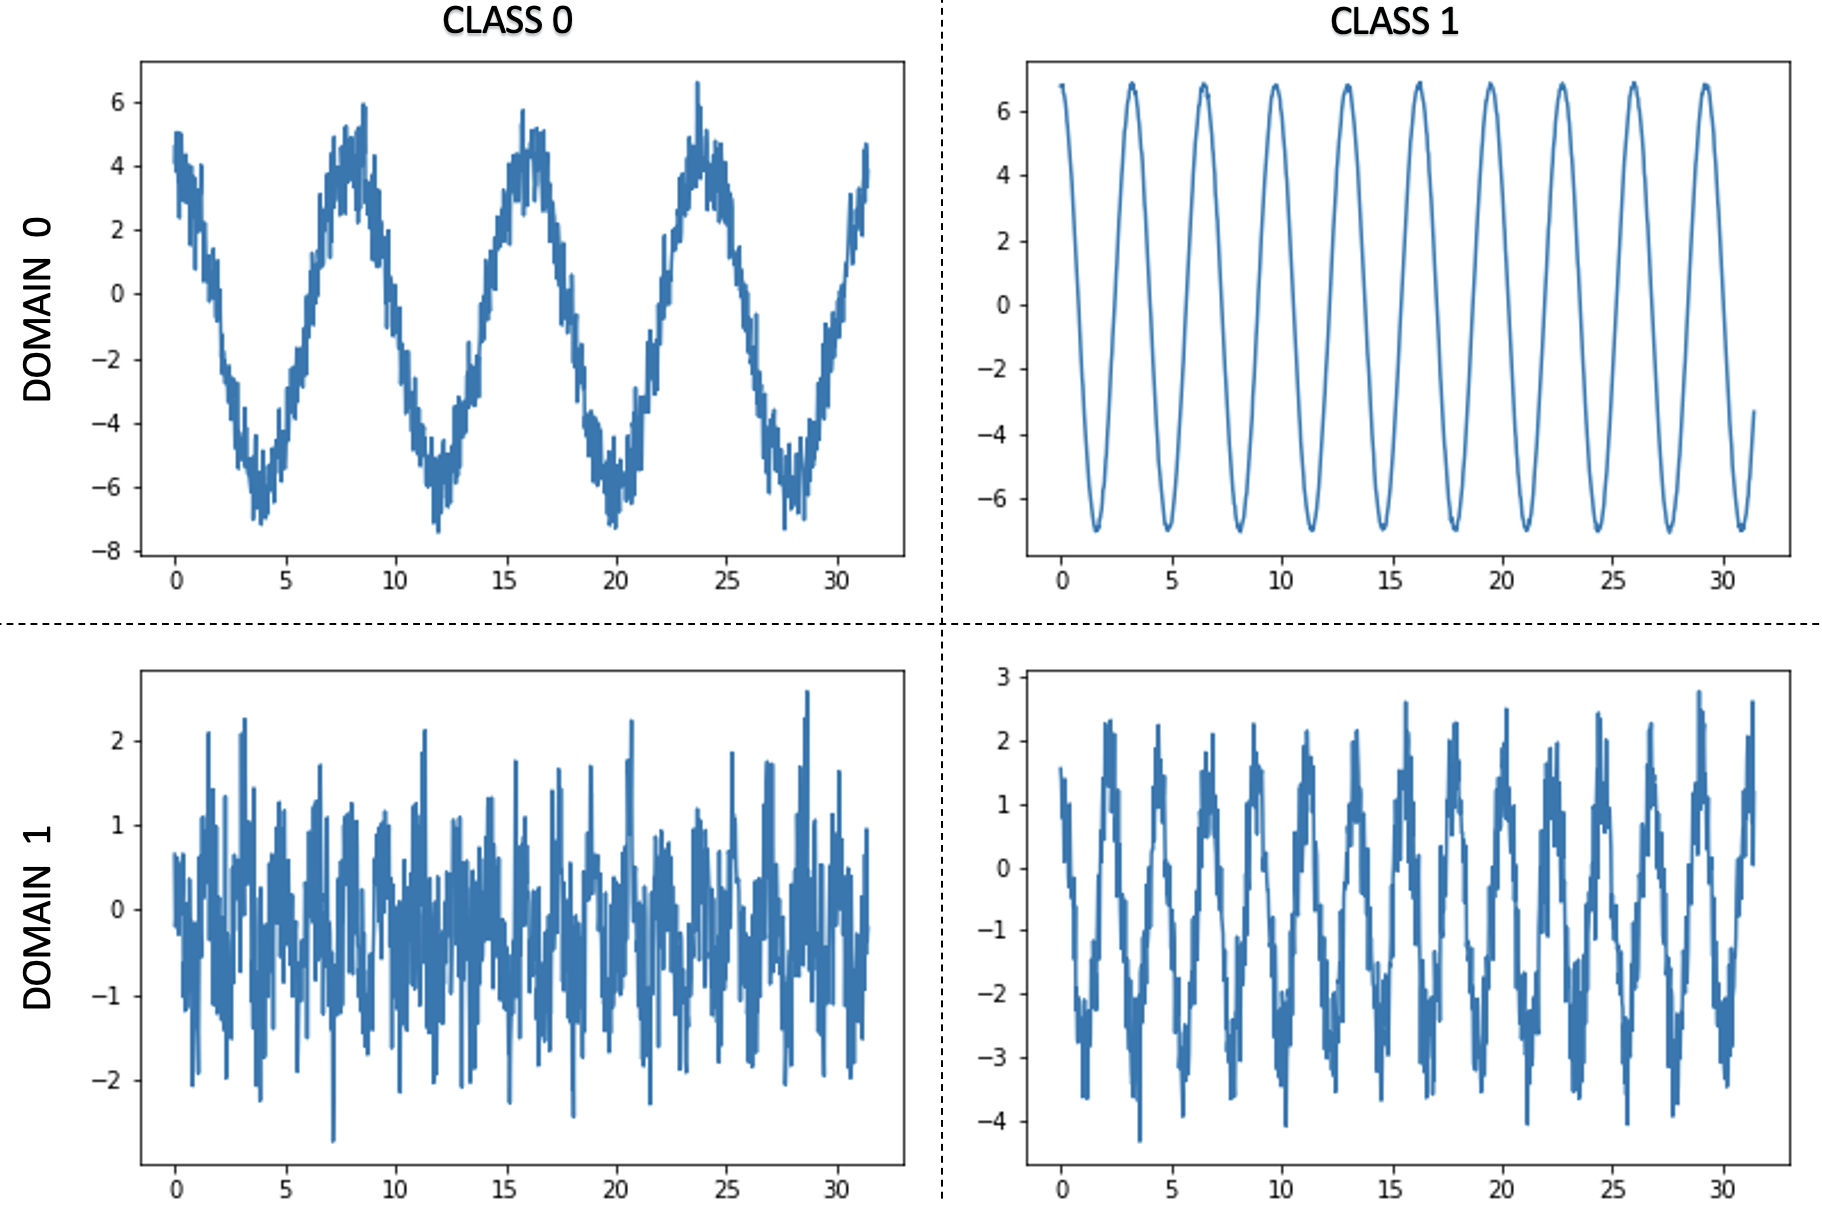
\includegraphics[width=0.9\textwidth]{samples_domain_class_dummy}
  \caption {Data Window Samples for each domain and class}
  \label{fig:samples_domain_class_dummy}
\end{figure}
\FloatBarrier 

In fig. \ref{fig:samples_domain_class_dummy_influence_noise} one can see how the applied perturbation and noise during the sampling process changes the data sequences belonging to the same class and domain. 


\begin{figure}[htpb]
  \centering
  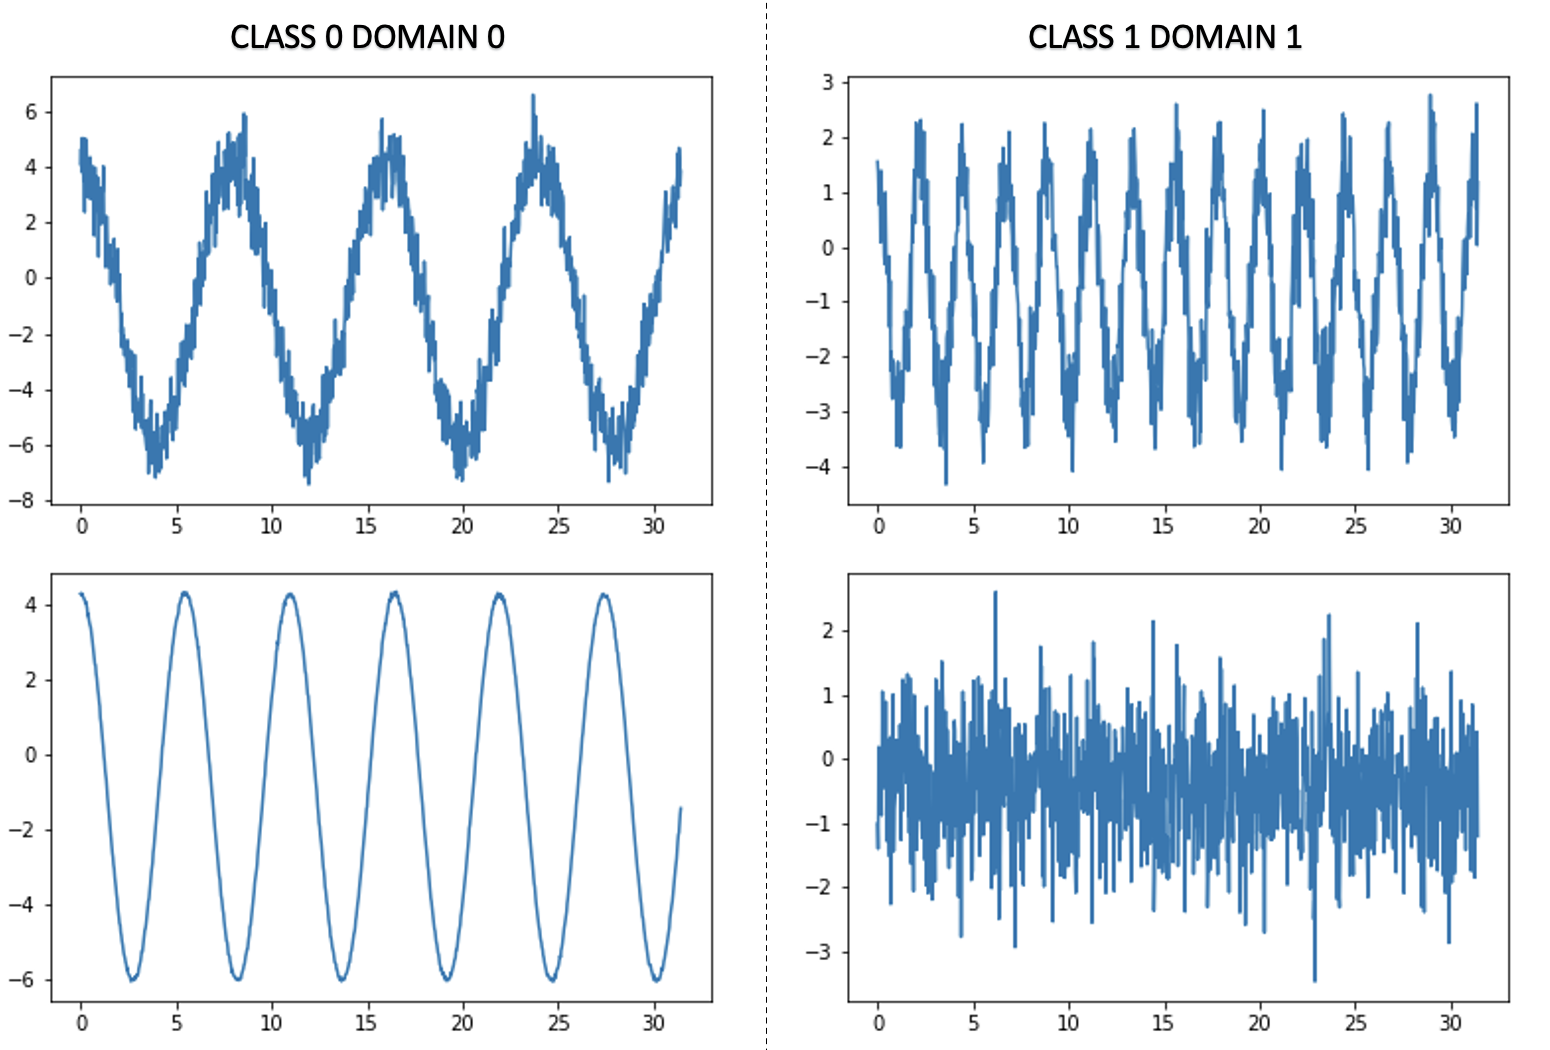
\includegraphics[width=0.9\textwidth]{samples_domain_class_dummy_influence_noise}
  \caption {Influence of perturbation when sampling several data sequences for one class and domain}
  \label{fig:samples_domain_class_dummy_influence_noise}
\end{figure}
\FloatBarrier 



\section{Proposed training with MMD and cross entropy loss} \label{sec:Proposed_training}

For the trainig of the deep-learning based domain adaption model a combination of cross-entrop and MMD loss is used. The repetitive training of the model is visualized in fig. \ref{fig:Training_Process_MMD}. For training the model data from the target and source domain is used in parallel. Firstly, the data used for the training is preprocessed. This step includes the collection, sorting and windowing of the data from different data sources. Also wavelet or fourier transforms can be included in order to generate more informative data for the model. The model used for predictive maintenance is concluded of a CNN and a classifier. In a first step the 1D CNN extracts expressive features, which are subsequently fed into a fully connected network to predict the health condition classes of each sample. The MMD loss estimates the discrepancy between latent feature vectors of source and target domain samples in several layers of the neural network. Source and target domain samples are grouped up in pairs of two. For each such randomly grouped latent feature vectors the MMD loss is calculated. Besides that the cross entropy loss, which is applied in the final layer evaluates the classification performance of the network. Fig. \ref{fig:MMD_Loss_and_CE_loss} symbolically shows how the MMD as well as the source cross-entropy loss is extracted from the different layers of the model.

\begin{figure}[htpb]
  \centering
  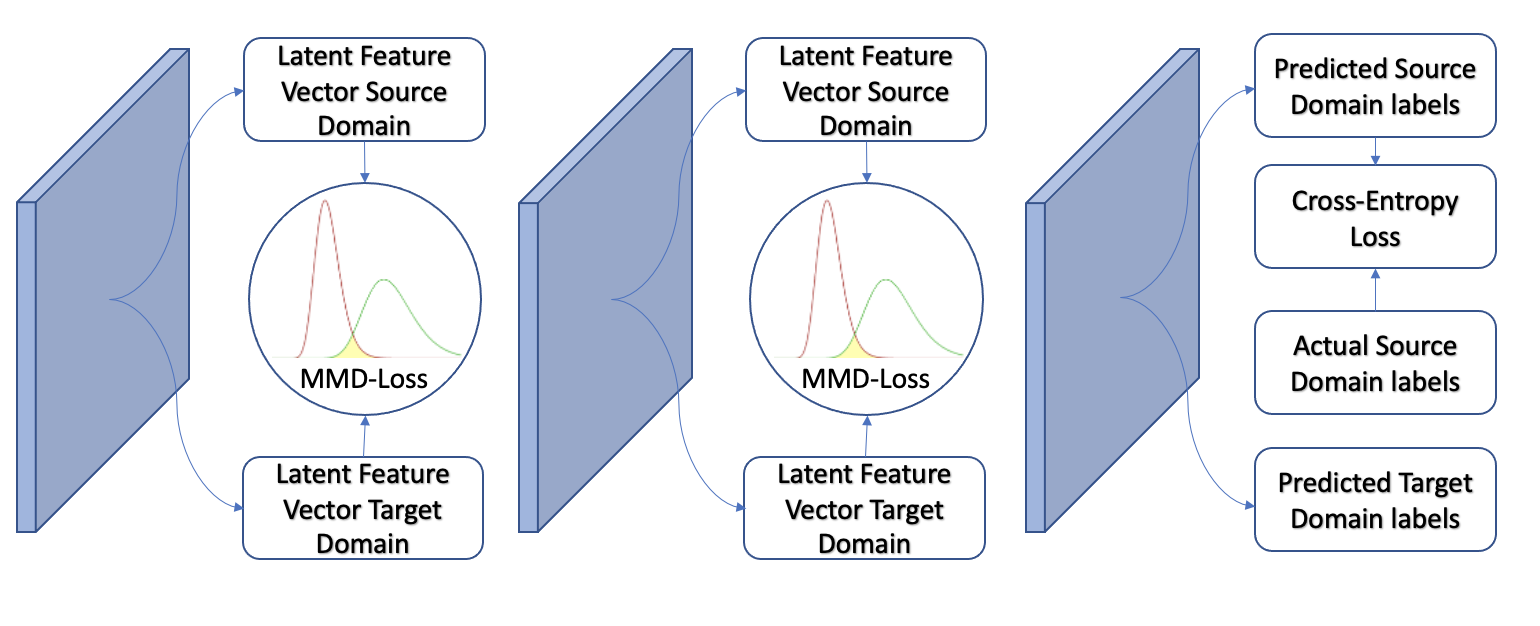
\includegraphics[width=1\textwidth]{MMD_loss_visualization}
  \caption {Cross Entropy Loss and MMD Loss in Neural Networks} \label{fig:MMD_Loss_and_CE_loss}
\end{figure}
\FloatBarrier 


Due to the MMD loss the model learns to extract features which are domain independent. By applying a source cross-entropy loss, the model learns to predict correct labels for the source domain samples.

The cross entropy loss is used to solve the classification problem. The MMD loss reduces the domain discrepancy, by extracting features which are more domain independent. When including several losses, a weighted average must be defined in order to train neural networks. These weighting factors are hyperparameters which need to be defined before training. The following equation presents the weighted average between cross entropy and MMD loss, which is used to optimize the model:

\begin{align}
    \mbox{Total Loss} = \mbox{Source Cross-Entropy Loss} + \mbox{GAMMA} * \mbox{MMD Loss}
\end{align}

In general the training is repeated until the maximum number of epochs is reached. After the training is completed the model can be used to predict the health labels for the target domain data. 

\begin{figure}[htpb]
  \centering
  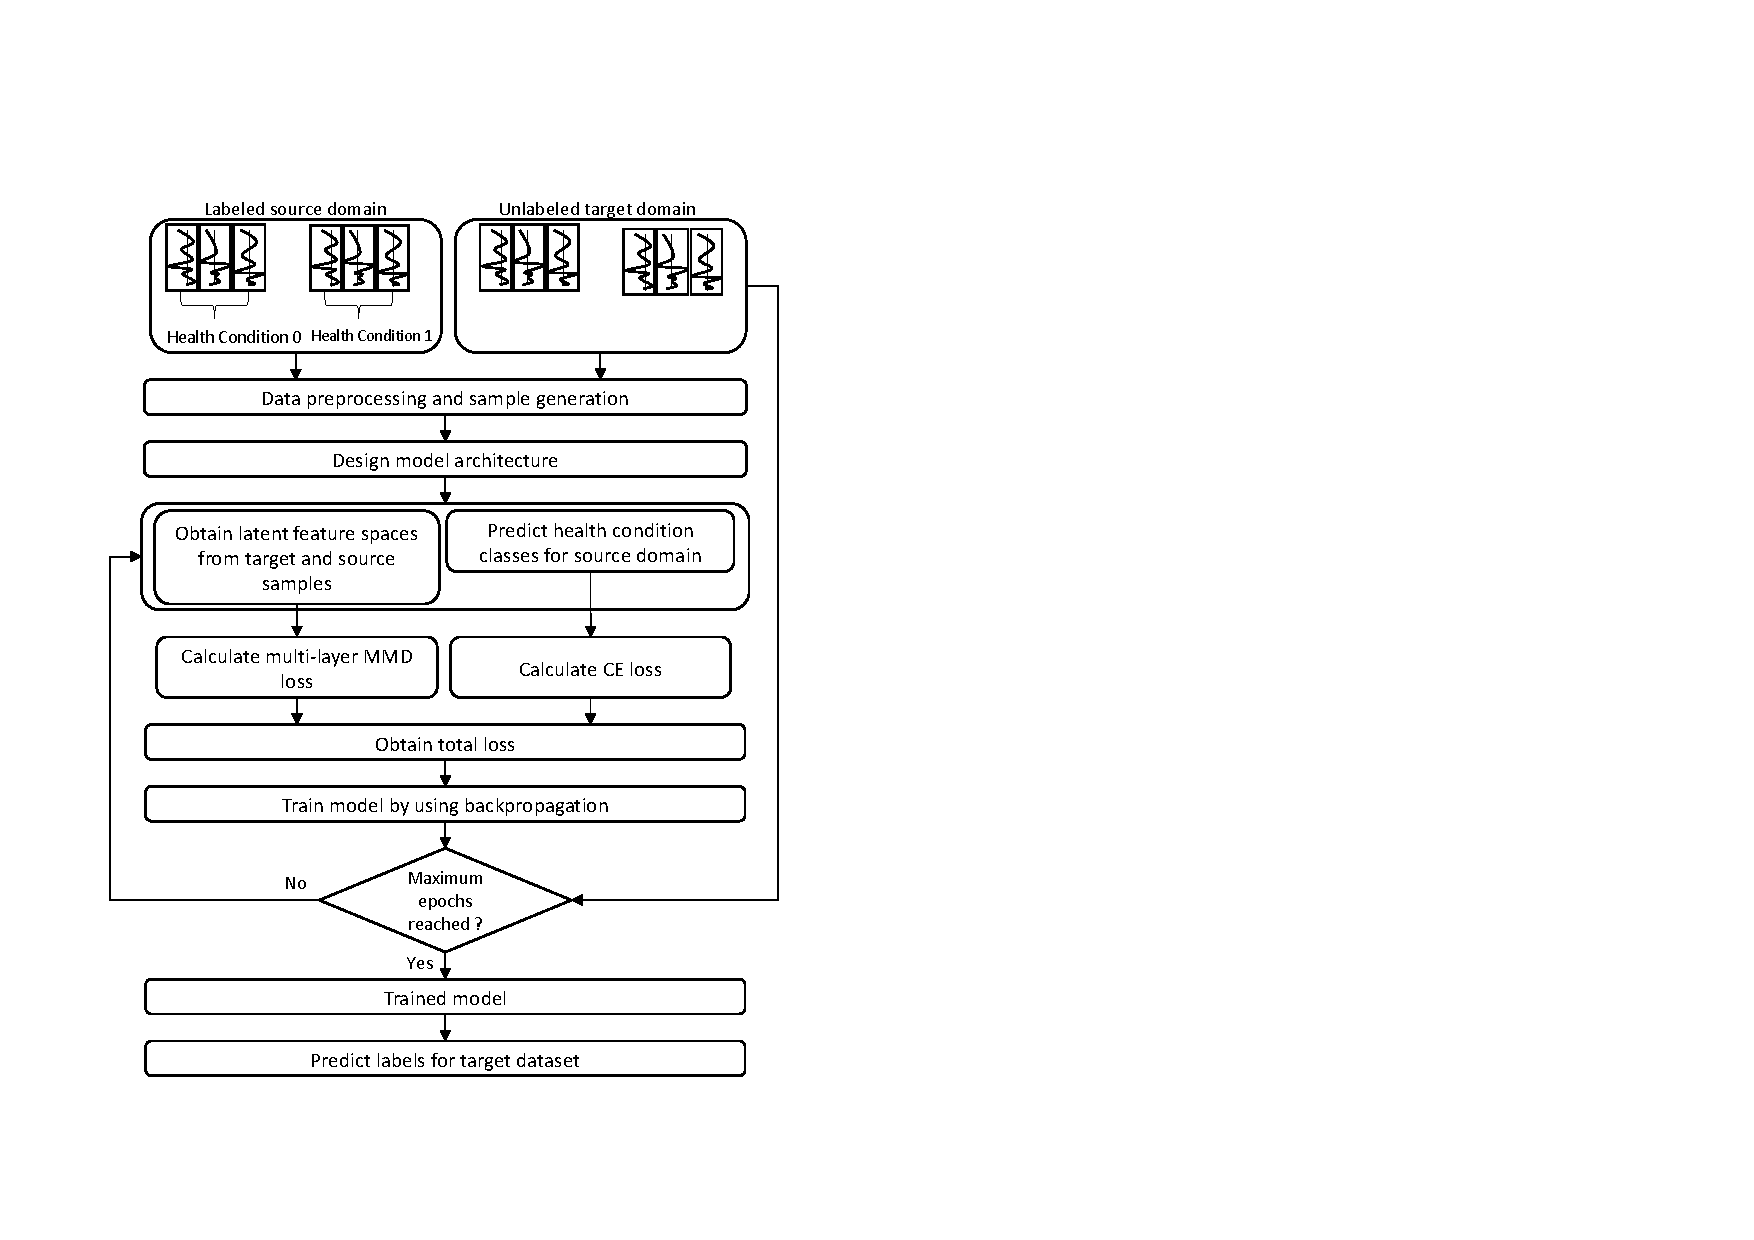
\includegraphics[width=0.8\textwidth]{training_process_mmd.pdf}
  \caption {Model training iteration} \label{fig:Training_Process_MMD}
\end{figure}
\FloatBarrier 

\section{Model}
In the MMD experiments different model architectures and optimizer were used. Generally the model consist of a 1D CNN which is responsible to extract expressive features. The CNN consists of 3 convolutional layers. With increasing depth of the network the kernel size decreases. This helps to extract more general and global features in shallow and more specific and local features in deeper layers. Depending of the underlying data complexity in the different experiments max pooling layers are included in order to avoid overfitting and exploding gradients. Including batch normalization after convolutional layers helps to make the training faster and more stable. This is done by fixing the means and variances of the layers inputs for each batch. After iteratively applying these three types of layers the output of the CNN is flattend to a 1D vector. This vector is used as an input for the subsequent classifier. The latent space size of the Classifier is reduced in each layer. The 2D output of the neural network represents the prediction probability for the two health condition classes.

